% !TEX root = ../report.tex

\chapter{The Chain-of-Integrators ADC}
\label{sec:ciadc}
The simplest control-bounded ADC is the Chain-of-integrators ADC, as presented in \cite{cbc_2020_loeliger}. This architecture consists of an integrator chain, where each integrator is stabilized by a local, independent digital control loop. A reader that is familiar with $\sd$ converters, might recognize this structure as very similar to a MASH $\sd$ modulator, and it is shown in \cite{malmberg_thesis} that the performance is also very similar. A block diagram of the full chain-of-integrators ADC is shown in figure \ref{fig:CI}.

This rather simple structure does not not utilize much of the mentioned design flexibility associated with control-bounded converters. However, the chain-of-integrators serves as an important starting point, and a thorough understand of its operating principle is helpful before considering more advanced architectures. The theoretical analysis is also rather straight forward and several important results from the analysis of the chain-of-integrators are directly applicable to other architectures. In addition, the simulations on the chain-of-integrators demonstrates the developed simulation framework which is an essential tool for further work on the topic.

This chapter is organized as follows. The first section presents a description of the analog system together with a transfer function analysis, based on the results from section \ref{sec:as_tf}. The digital control is then briefly described and the conditions for an effective control is discussed. Finally we present and discuss the simulation results.


\begin{figure}[hbp]
    \centering
    % !TEX root = ../../report.tex

\begin{tikzpicture}[scale=0.75, transform shape]
% --------------------- Nodes -------------------------------- %
\node[box] (I1) at (0,0) {\Large $\nicefrac{\beta}{s}$};
\node[box] (I2) at (5,0) {\Large $\nicefrac{\beta}{s}$};
\node[box] (IN) at (12,0) {\Large $\nicefrac{\beta}{s}$};

\node[circle, draw, inner sep=0.5mm] (add1) at (-2,0) {\Large+};
\node[circle, draw, inner sep=0.5mm] (add2) at (3,0) {\Large+};
\node[circle, draw, inner sep=0.5mm] (add3) at (10,0) {\Large+};

\node[box, anchor=north west, scale=0.8, transform shape] (SH1) at (1,-1.5) {S/H};
\node[box, anchor=north west, scale=0.8, transform shape] (Q1) at (0,-1.5) {\onebitqrev};
\node[box, anchor=north west, scale=0.8, transform shape] (DAC1) at (-1.5,-1.5) {D/A};

\node[box, anchor=north west, scale=0.8, transform shape] (SH2) at (6,-1.5) {S/H};
\node[box, anchor=north west, scale=0.8, transform shape] (Q2) at (5,-1.5) {\onebitqrev};
\node[box, anchor=north west, scale=0.8, transform shape] (DAC2) at (-1.5+5,-1.5) {D/A};

\node[box, anchor=north west, scale=0.8, transform shape] (SHN) at (6+7,-1.5) {S/H};
\node[box, anchor=north west, scale=0.8, transform shape] (QN) at (5+7,-1.5) {\onebitqrev};
\node[box, anchor=north west, scale=0.8, transform shape] (DACN) at (-1.5+5+7,-1.5) {D/A};

\node[box, minimum width=14.5cm, anchor=north west] (DE) at (-1.5,-4){Digital Estimator};

% \node[draw, dashed, minimum width=17cm, minimum height=2.5cm, anchor=north west](AS) at (-2.5, 1.8){};
% \node[yshift=-5mm] at (AS.north) {Analog System};

% \node[draw, dashed, minimum width=17cm, minimum height=2.5cm, anchor=north west](AS) at (-2.5, -0.8){};


% --------------------- Nodes -------------------------------- %
\draw[arrow] (-3,0) node[left]{$u(t)$} to[short, o-] (add1.west);
\draw[arrow] (add1.east) -- (I1.west);
\draw[arrow] (I1.east) -- (add2.west);
\draw[arrow] (add2.east) -- (I2.west);
\draw[] (I2.east) -- ++(2,0) node[anchor=west, minimum width=1cm](dots){$\cdots$};
\draw[arrow] (dots.east) -- (add3.west);
\draw[arrow] (add3.east) -- (IN.west);
\draw[arrow] (IN.east) -| (SHN.north)  node[above, xshift=6mm]{$\tilde{s}_N(t)$};
\node[above, xshift=1cm] at (IN.east) {$x_N(t)$};

\draw[] (SHN.west) -- (QN.east);
\draw[] (QN.west) -- (DACN.east)node[midway](sN){};
\draw[arrow] (DACN.west) node[below, xshift=-5mm]{$s_N(t)$} -| (add3.south);
\draw[arrow] (sN.center) to[short, *-] ++(0,-2.1) node[right, yshift=7mm]{$s_N[k]$};

\draw[arrow] (SH2.north) ++(0,1.5) node[above]{$x_1(t)$} to[short, *-] (SH2.north) node[above, xshift=6mm]{$\tilde{s}_1(t)$};
\draw[] (SH2.west) -- (Q2.east);
\draw[] (Q2.west) -- (DAC2.east)node[midway](s2){};
\draw[arrow] (DAC2.west) node[below, xshift=-5mm]{$s_1(t)$} -| (add2.south);
\draw[arrow] (s2.center) to[short, *-] ++(0,-2.1) node[right, yshift=7mm]{$s_1[k]$};


\draw[arrow] (SH1.north) ++(0,1.5) node[above]{$x_0(t)$} to[short, *-] (SH1.north) node[above, xshift=6mm]{$\tilde{s}_0(t)$};
\draw[] (SH1.west) -- (Q1.east);
\draw[] (Q1.west) -- (DAC1.east) node[midway](s1){};
\draw[arrow] (DAC1.west) node[below, xshift=-5mm]{$s_0(t)$} -| (add1.south);
\draw[arrow] (s1.center) to[short, *-] ++(0,-2.1) node[right, yshift=7mm]{$s_0[k]$};

\draw[arrow] (DE.south) -- ++(0,-1) node[below]{$\hat{u}(t)$};


\end{tikzpicture}

    \caption{A block diagram of an $N$th order chain-of-integrators ADC}
    \label{fig:CI}
\end{figure}





\section{Analog System}
The analog system of the chain-of-integrators ADC is part of the block diagram shown in figure \ref{fig:CI}. The (ideal) integrators has a transfer function $\nicefrac{\beta}{s}$, and the parameter $\beta$ is referred to as the \textit{integrator gain}. The input signal $u(t)$ is passed through $N$ such integrators, each being controlled by a local, independent control loop. Note that the input signal and output estimates of this ADC are both scalars, as a multi-input chain-of-integrators would be nothing more than $L$ equal systems in parallel.

The system dynamics is described by the equation
\begin{equation}
    \label{eq:CI_state_space_eq}
    \dot{\bm{x}}(t) = \Amat_{CI}\xtv + \Bmat_{CI}u(t) + \Gmat_{CI}\stv.
\end{equation}
where the system matrix and the input matrix are given by
\begin{equation}
    \label{eq:ci_amat}
    \Amat_{CI} =
    \begin{pmatrix}
    0  \\
    \beta & 0 \\
    & \ddots & \ddots & \\
    & &  \beta & 0
    \end{pmatrix}
    \in \R^{N \times N}
\end{equation}
and
\begin{equation}
    \label{eq:ci_bmat}
    \Bmat_{CI} = \Tr{
    \begin{pmatrix}
        \beta & 0 & \cdots & 0
    \end{pmatrix}
    }
    \in \R^{N \times 1}
\end{equation}
respectively.

The $N$ dimensional state-vector $\xtv$ is observed directly by the local digital control, and the control observation matrix is given by
\begin{equation}
    \label{eq:ci_GmattildeT}
    \GmattildeT_{CI} = \eyen{N}.
\end{equation}
The output of the 1 bit D/A converter is given by
\begin{equation}
    s_i(t) =
    \begin{cases}
        \kappa, & \text{if } s_i[k]=1 \\
        -\kappa,& \text{if } s_i[k]=0,
    \end{cases}
\end{equation}
and $\kappa$ is referred to as the \textit{control gain}. The control matrix is given by
\begin{equation}
    \label{eq:ci_Gmat}
    \Gmat_{CI} =
    \begin{pmatrix}
        \kappa \beta \\
        & \ddots \\
        & & \kappa \beta
    \end{pmatrix}.
\end{equation}

As mentioned in chapter \ref{sec:cbadc}, the signal observation matrix $\CmatT$ maps the state vector $\xtv$ to the output vector $\ytv$. As this matrix is purely conceptual, it has no part in the physical implementation and may be chosen independent of the analog system. Typically one would choose to map either all or only the last state to the output, by choosing either
\begin{equation}
    \label{eq:ci_cmats}
    \CmatT_{CI_s} =
        \begin{pmatrix}
            0 & \cdots & 0 & 1
        \end{pmatrix}
        \in \R^{1 \times N}
\end{equation}
or
\begin{equation}
    \label{eq:ci_cmatm}
    \CmatT_{CI_m} = \eyen{N}.
\end{equation}
These different choices of $\CmatT$ results in what is referred to as single and multiple output reconstruction, respectively. Intuitively one would think that considering all internal states of the analog system in the estimation filter would give increased performance, and this is indeed the case. The computational complexity of the filter is also indifferent to the choice of $\CmatT$, so $\CmatT_{CI_m}$ is the natural choice for this matrix. The single output matrix is still considered in this thesis for the sake of a tractable analysis.


\subsection{Transfer Function Analysis}
For this scalar input ADC, the analog transfer function of \ref{eq:ATF_def} reduces to a column vector. Each element of the transfer function vector is given by
\begin{equation}
    G_k(\omega) = \prod_{\ell = 0}^{N-1} \frac{\beta}{j \omega}.
\end{equation}
Hence for the single output reconstruction,
\begin{equation}
    G_s(\omega) = \left( \frac{\beta}{\jw} \right)^N
\end{equation}
and
\begin{equation}
    \label{eq:atf_ci_single}
    \norm{G_s(\omega)}{2}^2 = |G_{N-1}(\omega)|^2 = \left(\frac{\beta}{\omega}\right)^{2N}.
\end{equation}
For multiple output,
\begin{equation}
    \norm{G_m(\omega)}{2}^2 = \frac{1- \left( \frac{\omega}{\beta} \right)^{2N}}{ \left( \frac{\omega}{\beta} \right)^{2N} \left( 1 - \frac{\omega^2}{\beta^2} \right) }.
\end{equation}

A comparison of the analog transfer function obtained from single and multiple output is shown in figure \ref{fig:atf_ci_m_vs_s}, for $\beta = 2\pi \cdot \SI{20}{\mega\hertz}$ and $N=5$. As the figure shows, the difference is mainly visible for frequencies above the unity gain of the integrators.

\begin{figure}[htbp]
    \centering
    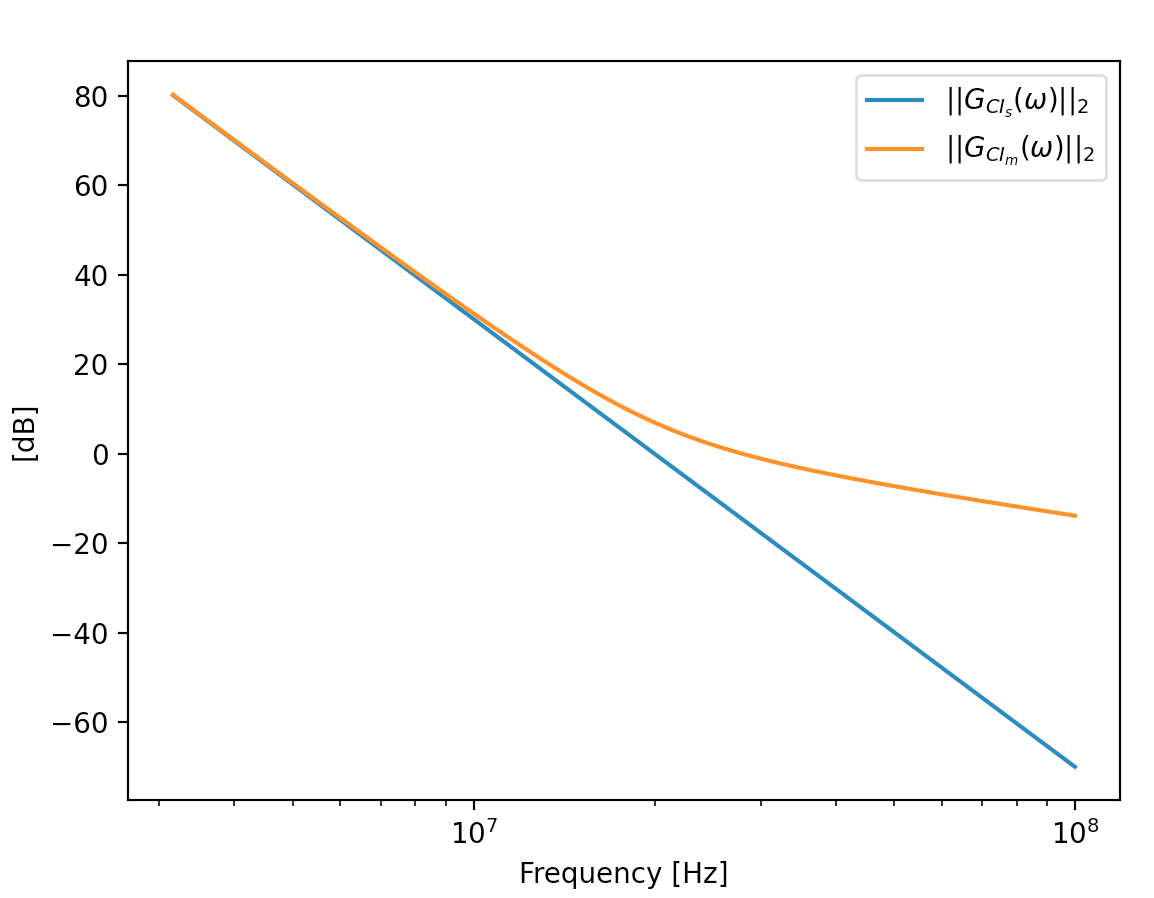
\includegraphics[width=\linewidth]{figures/051chain/ATF_m_vs_s.png}
    \caption{Comparison of analog transfer function obtained from single and multiple output, for $\beta = 2\pi \cdot \SI{20}{\mega\hertz}$ and $N=5$.}
    \label{fig:atf_ci_m_vs_s}
\end{figure}















\section{Effective digital control}
In the chain-of-integrators ADC, each integrator is under local digital control. This simple control structure is easy to implement and allows for an analytic derivation of the effective control criteria. This derivation is carried out in detail in \cite{malmberg_thesis} and the main results is presented here.

In the analysis, the input is assumed to be bounded, i.e. $|u(t)| \leq b_u \ \forall t$, and the conditions for effective control ensure $\norm{\xtv}{\infty} \leq b_{\bm{x}} \ \forall t$, see section \ref{sec:04digcontrol}. For the chain-of-integrators this is guaranteed If
\begin{equation}
    \label{eq:effctrl_kappa}
    |\kappa| \geq b_{\bm{x}}
\end{equation}
and
\begin{equation}
    \label{eq:effctrl_Tbeta}
    T|\beta|(|\kappa| + b_{\bm{x}}) \leq b_{\bm{x}}.
\end{equation}

\subsection{Implications on the Sampling Rate}
A natural choice of $\kappa$ and $b_{\bm{x}}$ is to let both equal the positive supply voltage. With $\kappa = \bx$, (\ref{eq:effctrl_Tbeta}) reduces to
\begin{equation}
    \label{eq:effctrl_simp}
    T|\beta| \leq \frac{1}{2}.
\end{equation}

To see how this condition influences the sampling rate, let $f_s = \frac{1}{T}$ be the sampling frequency of the digital control and let $f_u = \frac{\beta}{2 \pi}$ be the unity gain frequency of the integrators. Equation (\ref{eq:effctrl_simp}) may then be written as
\begin{equation}
    \label{eq:fs4fu}
    f_s \geq 4 \pi f_u,
\end{equation}
i.e. given $\kappa = \bx$, the sampling rate must be approximately $12.6$ times the unity gain frequency of the integrators in order to guarantee an effective control.

To place this requirement in the context of oversampling, the unity gain frequency must be related to the frequency band of interest. For simplicity, only the single output transfer function is now considered. Assume that the frequency content of the input signal is upper bounded by a frequency $f_0$ and the critical frequency of the estimation filter is set as $f_c \geq f_0$. From (\ref{eq:def_BW}) and (\ref{eq:atf_ci_single}), the parameter $\eta$ may be expressed as
\begin{equation}
    \label{eq:fu_vs_fc}
    \eta = \left(\frac{\beta}{\omega_c}\right)^{N} = \left( \frac{f_u}{f_c} \right)^N.
\end{equation}
Furthermore, from (\ref{eq:stf_eta_start})-(\ref{eq:stf_eta_end}), $\eta$ is also the relation between the magnitude of the signal and noise transfer function at the critical frequency. From (\ref{eq:fu_vs_fc}) it is seen that $\eta$ grows with system order as long as $\frac{f_u}{f_c} \geq 1$. We therefore define a practical limit
\begin{equation}
    f_u \geq 2f_c
\end{equation}
for this relation, in order to take advantage of the higher system order.

Based on this discussion the relation between the signal bandwidth $f_0$ and the sampling rate may ultimately be expressed as
\begin{equation}
    f_s \geq 8 \pi f_0,
\end{equation}
or equivalently
\begin{equation}
    \text{OSR} \geq 4\pi.
\end{equation}
Thus, for a reasonable chain-of-integrators ADC with guaranteed stability and $\kappa=\bx$, the minimum oversampling rate is approximately 12.6.

As mentioned in section \ref{sec:04digcontrol}, designing for stability guarantee is not attractive from a performance point of view. In section \ref{sec:practical_remarks} it was shown that $T, \beta$ and $\bx$ are the only parameters affecting the SNR of a control-bounded ADC and it is therefore an inevitable trade-off between stability and performance. The preferred way of determining this trade-off is by simulations, and the results obtained in this section serves as a useful starting point.















\section{Simulations}
The process of simulating a control-bounded ADC is divided into two separate steps. First, the interaction between the analog system and the digital control is simulated in time domain to generate the control signal $\skv$. In the following, this part of the simulation process is referred to as the \textit{system simulation}. These control signals are then applied as input to the digital estimation filter, which reconstructs the output estimate $\utvhat$. For the chain-of-integrators ADC, the system simulations are done using the Spectre simulation platform \cite{spectre} and the estimation filter is implemented offline in Python.

\subsection{System Simulation}
The circuit used for the system simulation is a 5th order system, derived from the block diagram of figure \ref{fig:CI}. The integrators are implemented using a first order opamp-RC filter as shown in figure \ref{fig:opampRCint}, and the opamp is modelled by an ideal voltage controlled voltage source.
\begin{figure}[htbp]
    \centering
    % !TEX root = ../../report.tex
\begin{circuitikz}

% Opamp
\node[op amp](opamp) at (2,0) {};

\draw (opamp.-) -- ++(-0.5, 0) node[](a){} -- ++(-0.5, 0) node[](b){} to[R, -o, l_=$R_{\beta}$] ++(-3,0) node[left]{$x_{k-1}(t)$};
\draw (b.center) to[short, *-] ++(0,2) to[R, -o, l_=$R_{\kappa\beta}$] ++(-3,0) node[left]{$s_{k}(t)$};

\draw (opamp.+) -- ++(0,-0.5) node[ground]{};
\draw (a.center) to[short, *-] ++(0,1.5) to[C, l=$C$] ++(2.5,0) -| (opamp.out) to[short, -*] ++(0,0);
\draw (opamp.out) to[short, -o] ++(1,0) node[right]{$x_k(t)$};

\end{circuitikz}

    \caption{An Opamp-RC integrator used for the chain-of-integrators simulation.}
    \label{fig:opampRCint}
\end{figure}
The Sample-and-hold, 1 bit quantizer and 1 bit dac, are all incorporated in an ideal, clocked comparator written in VerilogA. The digital control signal $\skv$ does therefore not exist in the system simulation and is extracted from the control contribution, $\stv$, in a post-processing step.

\subsection{Estimation Filter Implementation}
The digital estimation filter is implemented in Python and the source code is available at GitHub \cite{cbadcsim2}. The filter is first initialized by computing the offline matrices, defined by equations (\ref{eq:def_Af})-(\ref{eq:W_sys}). The actual estimate is then carried out recursively as described by (\ref{eq:mf})-(\ref{eq:uhat_filter_estimate}). As the recursive estimate takes place after the system simulation is complete, both the forward and the backward recursion uses all available control signals. In a production environment, this is obviously not possible and only a limited amount of \enquote{future} samples are available. The filter algorithm is quite sensitive to the boundary conditions, but usually a few hundred samples is enough for the filter to settle properly.

\subsection{Simulation Results}
The parameters used for the simulation is summarized in table \ref{tab:CI_params}. The integrator gain is achieved by choosing $R_{\beta} = \SI{320}{\kilo\ohm}$ and $C = \SI{10}{\femto\farad}$. The comparator output is $\pm \SI{1}{\volt}$, and the control gain is set to $\kappa=1$ by having $R_{\kappa\beta} = R_\beta$.
% !TEX root = ../../report.tex

\begin{table}[htbp]
  \centering
  \caption{Simulation parameters, Chain-of-Integrators}
    \begin{tabular}{lcc}
    \rowcolor[rgb]{ 0,  0,  0} \textcolor[rgb]{ 1,  1,  1}{\textbf{Parameter}}	 & \textcolor[rgb]{ 1,  1,  1}{\textbf{Symbol}}
                             & \textcolor[rgb]{ 1,  1,  1}{\textbf{Value}}              \\
    Critical frequency       & $f_c$            & $\SI{10}{\mega\hertz}$                  \\
    Unity gain frequency     & $f_u$            & $\SI{50}{\mega\hertz}$               \\
    Integrator gain          & $\beta$          & $\SI{315}{\mega\hertz}$               \\
    Sampling frequency       & $f_s$            & $\SI{650}{\mega\hertz}$                 \\
    Oversampling ratio       & $\text{OSR} \left( \frac{f_s}{2f_c} \right)$ & $32.5$     \\
    System order             & $N$              & $5$                                     \\
    Control gain             & $\kappa$          & $\SI{1}{\volt}$                                  \\
    State boundary (input boundary)  & $b_{\bm{x}}$ ($b_{\bm{u}}$)    & $\SI{1}{\volt}$ ($\SI{1}{\volt}$)       \\
    Input signal frequency   & $f_{in}$         & $\SI{650}{\kilo\hertz}$              \\
    Input signal amplitude   & $a_{in}$         & $\SI{0.9}{\volt}$

    \end{tabular}
  \label{tab:CI_params}
\end{table}




A plot of the estimated power spectral density is provided in figure \ref{fig:CI_sim_N5}, for both the single and multiple output case. Note that the difference is mainly notable for frequencies above the critical frequency of the estimation filter.
\begin{figure}
    \centering
    \includegraphics[width=\linewidth]{figures/051chain/CI_SIM_N5.png}
    \caption{Estimated PSD for a 5th order chain-of-integrator ADC. $CI_m$ and $CI_s$ refers to multiple and single output reconstruction respectively.}
    \label{fig:CI_sim_N5}
\end{figure}

% A snapshot of the time-domain simulation is shown in figure \ref{fig:snapshot_x1x5}, which compares the state signals $x_0(t)$ and $x_4(t)$ for a full scale sinusoidal input.  Note that the input signal is clearly present in $x_1(t)$, while it is almost invisible in $x_5(t)$.
% \begin{figure}[htbp]
%     \centering
%     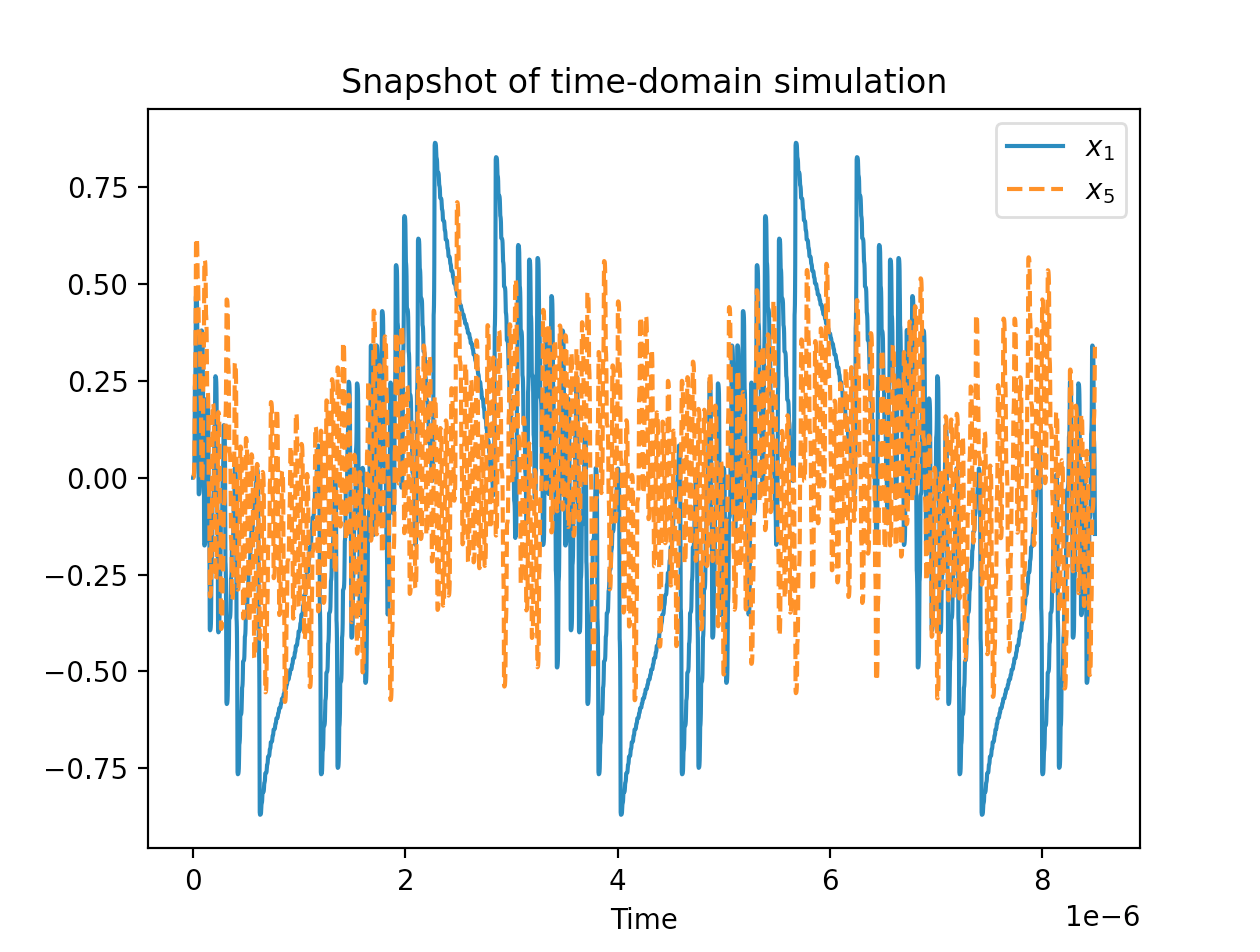
\includegraphics[width=\linewidth]{figures/051chain/CI_time_x1x5.png}
%     \caption{Time-domain snapshot of $x_1(t)$ and $x_5(t)$, for a full scale sinusoidal input.}
%     \label{fig:snapshot_x1x5}
% \end{figure}

% \begin{figure}[!ht]
%     \begin{subfigure}[b]{.5\linewidth}
%       \centering
%       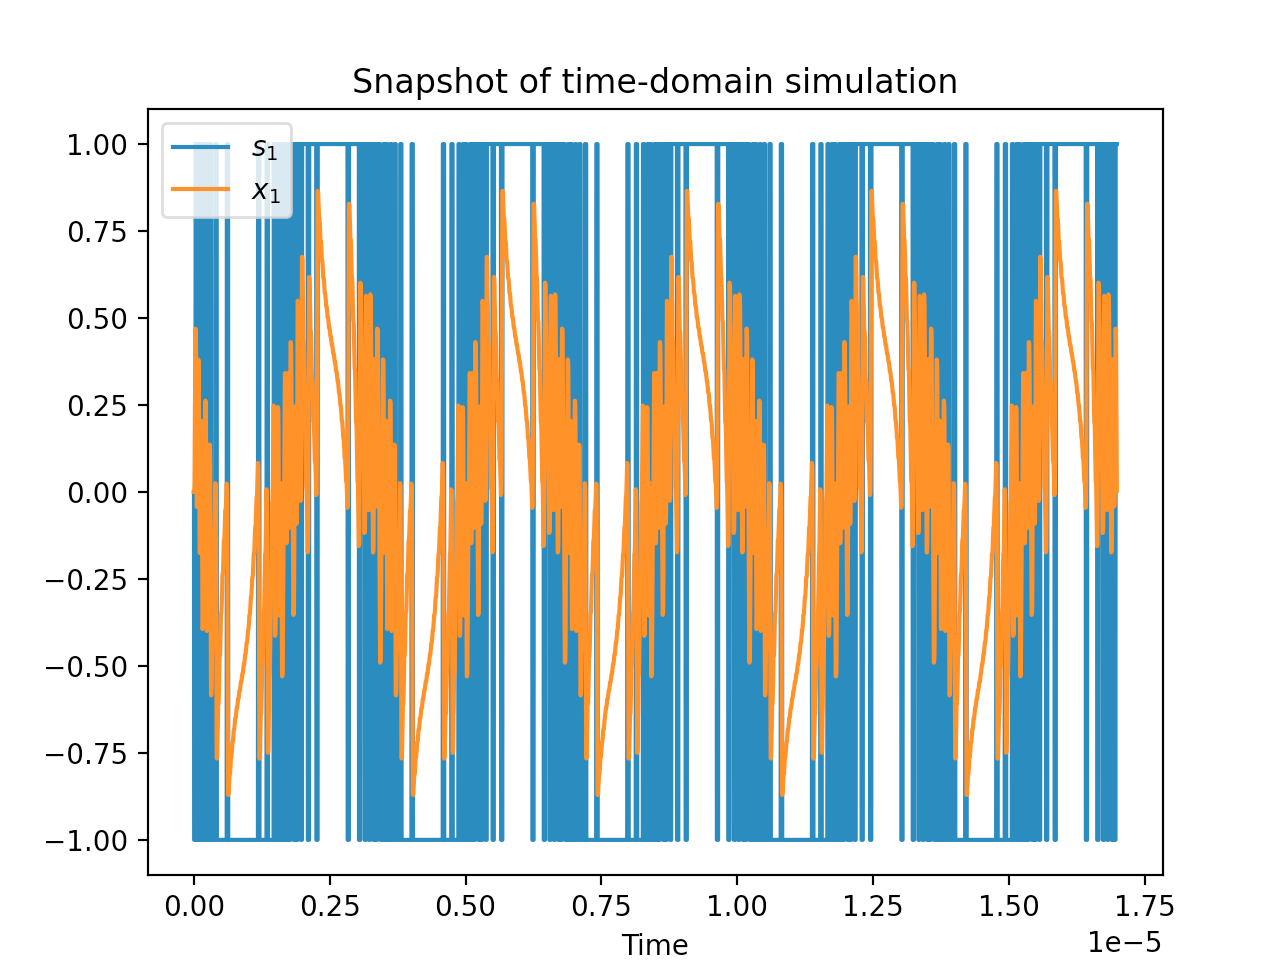
\includegraphics[width=\linewidth]{figures/051chain/CI_time_x1s1.png}
%       \caption{A subfigure}
%       \label{fig:1a}
%     \end{subfigure}%
%     \begin{subfigure}[b]{.5\linewidth}
%       \centering
%       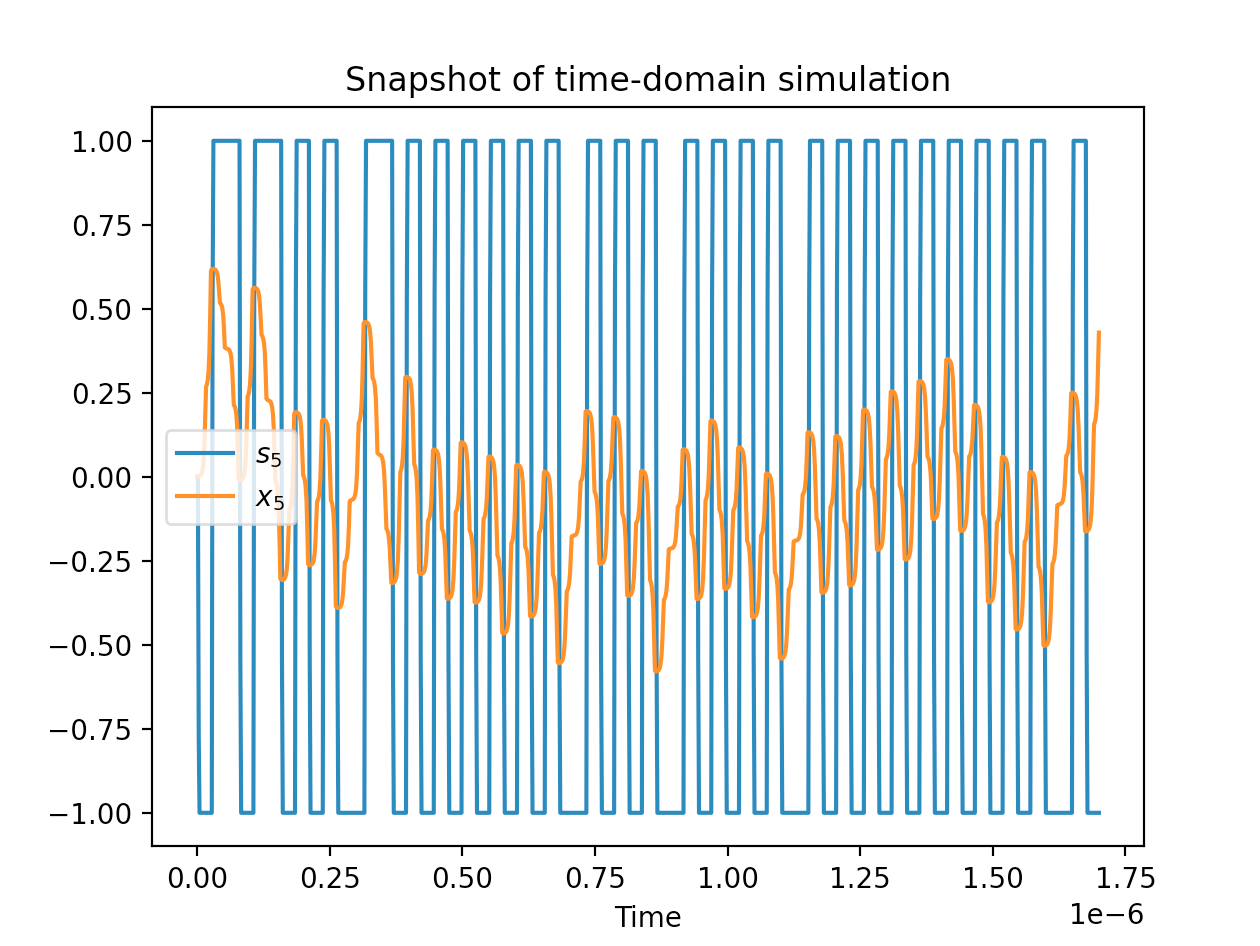
\includegraphics[width=\linewidth]{figures/051chain/CI_time_x5s5.png}
%       \subcaption{Another subfigure}
%       \label{fig:1b}
%     \end{subfigure}
%     \caption{A figure with two subfigures}
%     \label{fig:1}
%   \end{figure}
